\chapter{Индукция и рекурсия}

%rec: label prefix
Чтобы понять что такое \emph{рекурсия}, нужно понять, что такое \emph{рекурсия}. Для углубленного изучения вопросов, касающихся индукции и рекурсии, рекомендуются \cite{bib:haggard:discrmathprogrammer,bib:miller:secParAlghorithm,bib:hopkroft:automateIntro}.


\section{Индукция и рекурсия}

Термины \emph{индукция} и \emph{рекурсия} часто употребляются вместе. Следует провести границу между ними.

Математическая \emph{индукция} --- это метод рассуждений (доказательства) от частного к общему. То есть утверждения об общем случае выводятся(\emph{индуцируются}) из очевидных частных случаев --- \emph{фактов}. Базовый принцип математической индукции заключается в следующем.
\begin{enumerate}
    \item \emph{Базис}. Показана истинность утверждения $P(i)$, где $i\in\mathbb{N}$. Обычно $i=0$ или $i=1$. Но в общем случае может быть и так, что $P(j)$ ложно для $j<i$.
    \item \emph{Индуктивный переход}. Для произвольного $n\geq i,n\in\mathbb{N}$ доказано, что из истинности $P(n)$ следует истинность $P(n+1)$. Т.е. доказываем $P(n)\Rightarrow P(n+1)$.
\end{enumerate}

\begin{exampl}
    Задача. Доказать, что 
    \[
        \sum_{i=0}^{n}i^2=\frac{2n^3+3n^2+n}{6}.
    \]
\end{exampl}
\begin{proof}[Решение]
    В качестве базисного случая возьмем $n=0$. Видно, что равенство выполняется.
    
    По индукции предположим $n\geq 0$. Подставим вместо $n$ значение $n+1$:
    \[
        \sum_{i=0}^{n+1}i^2=\frac{2n^3+9n^2+13n+6}{6}.
    \]
    
    Справедливо:
    \[
        \begin{split}
            \sum_{i=0}^{n+1}i^2=(n+1)^2+\sum_{i=0}^{n}i^2=\\
            =(n+1)^2+\frac{2n^3+3n^2+n}{6}=\frac{2n^3+9n^2+13n+6}{6}.
        \end{split}
    \]
    Следовательно, можно сделать вывод, что доказываемое утверждение спрведливо для всех $n$.
\end{proof}

Общая форма математической индукции заключается в следующем.
\begin{enumerate}
    \item \emph{Базис}. Показана истинность утверждений $P(i),P(i+1),\ldots,P(j)$, где $i,j\in\mathbb{N},j>i$.
    \item \emph{Индуктивный переход}. Для $n\geq j$ при доказательстве истинности $P(n+1)$ можно использовать не только $P(n)$, но и все утверждения $P(i),P(i+1),\ldots,P(n)$.
\end{enumerate}

\begin{exampl} 
    Задача. Доказать $P(n)$: если $n\geq 8$, то $n$ можно представить суммой троек и пятерок.
\end{exampl}
\begin{proof}[Решение]
    Базис: 8=3+5, 9=3+3+3, 10=5+5. Индуктивный переход. Предполагаем истинность $P(8),P(9),P(10),\ldots,P(n)$. Доказывая $P(n+1)$ вычтем $3$ из $n+1$. Заметим, что $P(n-2)$ истинно. То есть $n-2$ представимо суммой $3k+5m$ пятерок и троек, а стало быть и $n+1$ также представимо, так как $n+1=3(k+1)+5m$.
\end{proof}

\emph{Рекурсия} в общем случае --- это \emph{самоподобие}. Таким свойством самоподобности, кроме всех прочих объектов, могут обладать математические формулы, данные и алгоритмы. 

Примером рекурсивной (самоподобной) структуры данных может быть список.
\begin{exampl} 
    Пусть имеются атомарные (неделимые) типы данных, такие как: число, строка, символ и т.д. Список можно определить так:
    \begin{enumerate}
        \item любой атом есть список;
        \item если $l_1,l_2,\ldots,l_n$ --- списки, то $(l_1,l_2,\ldots,l_n)$ есть список;
        \item ничто другое не является списком.
    \end{enumerate}
    
    Пример списка: $(1,(2,(3,4)),5)$.\qed
\end{exampl}

Рекурсивный алгоритм решения задачи обычно выполняется так:
\begin{enumerate}
    \item если задача тривиальна, то выдается решение и алгоритм завершается;
    \item в противном случае исходная задача разбивается на подзадачи меньшей размерности;
    \item каждая подзадача, решается тем же алгоритмом, что и исходная задача (то есть \emph{рекурсивно});
    \item решения подзадач объединяются так, чтобы получить решение исходной задачи.
\end{enumerate}

Важно отметить следующие особенности рекурсивных алгоритмов.
\begin{enumerate}
    \item Существование одного или нескольких базовых случаев для решаемой задачи. Решение базового случая тривиально и может быть получено сразу. Именно к базовым случаям в конечном итоге сводится решение любой исходной задачи.
    \item Существование способа сведения исходной задачи к решению подобных ей подзадач и получения результата исходной задачи на основе результатов подзадач.
\end{enumerate}

Индуктивные рассуждения часто используются для обоснования корректности рекурсивных алгоритмов. Самоподобные (рекурсивные) логические рассуждения называются индуктивными.


\section{Реккурентные математические формулы}

Выражающиеся сами через себя математические формулы называют \emph{реккурентными}. Вычисление значений таких формул для больших $n$ занимает слишком много времени, поэтому представляет интерес возможность свести реккурентность к <<замкнутой>> (аналитической) формуле, то есть к вычислимой непосредственно. Для рассматриваемых ниже реккурентных формул первого и второго рода порой удается получить решение в <<замкнутой форме>>.


\subsection{Реккурентные формулы первого рода}

В качестве примера рассмотрим задачу о Ханойских башнях.
\begin{exampl} 
    Задача. На первый из трех алмазных стержней насажены золотые диски в количестве 64-х штук. Все диски разного диаметра и диск меньшего диаметра лежит на диске большего диаметра. Требуется переместить диски на третий стержень в том же порядке, в каком они находятся на первом, перекладывая за раз по одному диску. Второй столбик используется как вспомогательный. В процессе перемещения нельзя класть больший диск на меньший\footnote{По легенде задача поставлена Всевышним перед жрецами, которые в настоящий момент над ней должны работать в несколько смен днем и ночью, и как только они закончат, наступит конец света. Хотелось бы прикинуть: стоит ли вообще браться за дальнейшее изучение рекурсии?}.
\end{exampl}
\begin{proof}[Решение]
    Возьмем меньшее количество дисков и убедимся, что задача решаема (см. рис \ref{fig:rec:hanoi}). Для одного диска решение очевидно. Для двух тоже.

    \begin{figure}
        \centering
        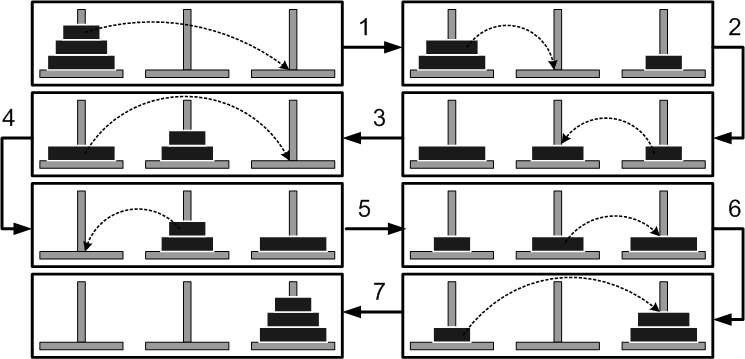
\includegraphics[width=0.67\textwidth]{fig/hanoi.png}
        \caption{Ханойские башни (три диска)}\label{fig:rec:hanoi}
    \end{figure}

    Попробуем обобщить на произвольное количество дисков. Для того, чтобы перенести $n$ дисков на третий столбик нужно $n-1$ верхних дисков сложить на второй столбик (очевидно, это можно сделать), оставшийся на первом столбике диск переложить на третий, и на него переместить $n-1$ дисков со второго (см. рисунок \ref{fig:rec:hanoi4}).

    \begin{figure}
        \centering
        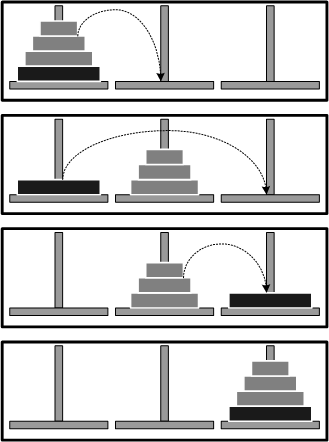
\includegraphics[width=0.27\textwidth]{fig/hanoi4.png}
        \caption{Ханойские башни (обобщение)}\label{fig:rec:hanoi4}
    \end{figure}

    Стало быть, если $T(n)$ --- количество перекладываний для переноса $n$ дисков, имеем: перенос на второй столбик потребует $T(n-1)$ перекладываний, одно перекладывание с первого на третий, и финальные $T(n-1)$ перекладываний на третий. $T(n)=2\cdot T(n-1) + 1$. В реккурентной форме:
    \[
        T(n)=
        \begin{cases}
            0,                  & n=0, \text{\emph{База рекурсии}},\\
            2\cdot T(n-1) + 1,  & n>0, \text{\emph{Реккурентный переход}}.
        \end{cases}
    \]

    Теперь можно легко двигаться от базы, получая:
    \[
        \begin{array}[c]{c||c|c|c|c|c|c|c|c|c|}
            \hline
            n       &0  &1  &2  &3  &4  &5  &6  &7   &8\\ \hline
            T(n)    &0  &1  &3  &7  &15 &31 &63 &127 &255\\ \hline
        \end{array}
    \]

    Тем не менее это неудобно --- слишком много последовательных решений. Хотелось бы сразу, не впадая в рекурсивный спуск, ответить сколько же нужно перекладываний для перемещения $n$ дисков? Пусть $K(n)=T(n)+1$.

    \[
        \begin{split}
                        T(n)+1=2\cdot T(n-1) + 2\Rightarrow\\
            \Rightarrow T(n)+1=2\cdot (T(n-1) + 1)\Rightarrow\\
            \Rightarrow K(n)=2\cdot (K(n-1))\Rightarrow\\
            \Rightarrow K(n)=2\cdot 2\cdot (K(n-2))\Rightarrow\\
            \Rightarrow K(n)=\underbrace{2\cdot 2\cdot\ldots\cdot 2\cdot2}_{n}\cdot K(0) = 2^n\Rightarrow\\
            \Rightarrow T(n)=K(n)-1=2^n-1.
        \end{split}
    \]

    Решение задачи о Ханойских башнях\footnote{Возвращаясь к теме конца света: если Всевышний запретил жрецам использовать роботов, то шанс разобраться с рекурсией есть}: $T(64)=2^{64}-1=18446744073709551615$ перекладываний.
\end{proof}

К сожалению, не всегда получается перейти от реккурентной формулы к простой аналитической, как это сделано в задаче о Ханойских башнях. В общем случае реккурентные формулы первого рода определяются так:
\begin{equation}
    \label{eq:rec:rec1type}
    T(n)=
    \begin{cases}
        f(k),                  & n=k, \text{\emph{База рекурсии}},\\
        c\cdot T(n-1) + f(n),  & n>k, \text{\emph{Реккурентный переход}},
    \end{cases}
\end{equation}
где $n,k\in\mathbb{N}$, $c$ --- константа, а $f$ --- ненулевая функция от $n$ при $n\geq k$.

При этом формуле \eqref{eq:rec:rec1type} эквивалентна сумма
\begin{equation}
    \label{eq:rec:rec1typeSum}
    T(n)=\sum_{i=k}^{n}c^{n-i}\cdot f(i).
\end{equation}

Это можно доказать по индукции, или выполнив $n-k$ подстановок вместо $T(n-1)$ в выражении реккурентного перехода формулы \eqref{eq:rec:rec1type}. Программисту эта эквивалентность дает возможность уйти от рекурсивной подпрограммы к обычному циклу.


\subsection{Реккурентные формулы второго рода}

Примером реккурентных формул второго рода являются числа Фибоначчи, определяемые рекурсивно так:
\begin{equation}
    \label{eq:rec:fibonacci}
    f(n)=
    \begin{cases}
        0,              &n=0\\
        1,              &n=1\\
        f(n-1)+f(n-2),  &n\geq 2.
    \end{cases}
\end{equation}

В общем случае реккурентные формулы второго рода имеют вид
\begin{equation}
    f(n)=
    \begin{cases}
        a_{k},                          &n=k\\
        a_{k+1},                        &n=k+1\\
        b_1\cdot f(n-1)+b_2\cdot f(n-2),&n\geq k+2,
    \end{cases}
\end{equation}
где $b_1,b_2$ --- константы.

Алгоритм получения аналитического решения для данных соотношений следующий.
\begin{enumerate}
    \item Предположив $f(n)=c^n$, подставить выражение в формулу реккурентного перехода $f(n)=b_1\cdot f(n-1)+b_2\cdot f(n-2)$: 
    \[
        \begin{split}
                        c^n-b_1\cdot c^{n-1}-b_2\cdot c^{n-2} = 0\Rightarrow\\
            \Rightarrow c^{n-2}\cdot(c^2 - b_1\cdot c - b_2) = 0.
        \end{split}
    \]
    
    \item Решить\footnote{Напомним, что для квадратного уравнения $ax^2+bx+c=0$ решениями будут $x_{1,2}=\frac{-b\pm\sqrt{b^2-4ac}}{2a}$} характеристическое уравнение $c^2 - b_1\cdot c - b_2 = 0$ относительно $c$, получив корни $c_1,c_2$.
    
    \item $f(n)$ будет имет следующее аналитическое выражение:
    \begin{equation}
        \label{eq:rec:rec2typeAnalytic}
        f(n)=D_1\cdot {c_1}^n + D_2\cdot{c_2}^n,
    \end{equation}
    где $D_1,D_2$ --- параметры, которые необходимо найти.
    
    \item Воспользоваться начальными условиями, чтобы построить систему уравнений
    \[
        \begin{cases}
            a_k     = D_1\cdot {c_1}^k + D_2\cdot{c_2}^k\\
            a_{k+1} = D_1\cdot {c_1}^{k+1} + D_2\cdot{c_2}^{k+1}\\            
        \end{cases}
    \]
    
    Решить систему относительно двух неизвестных $D_1,D_2$.
    
    \item Решением реккурентности будет формула \eqref{eq:rec:rec2typeAnalytic}.
\end{enumerate}

\begin{exampl}
    Найти аналитическое решение для поиска чисел Фибоначчи (см. формулу \eqref{eq:rec:fibonacci}).
\end{exampl}
\begin{proof}[Решение] 
    Применяя алгоритм:
    
    \begin{enumerate}
        \item Характеристическое уравнение $c^2-c-1=0$.
        \item Корни характеристического уравнения: $c_1=\frac{1+\sqrt{5}}{2},c_2=\frac{1-\sqrt{5}}{2}$
        \item Решая систему уравнений:
        \[
            \begin{cases}
                0=D_1 + D_2\\
                1=D_1\frac{1+\sqrt{5}}{2} + D_2\frac{1-\sqrt{5}}{2},
            \end{cases}
        \]
        получаем решения $D_1=\frac{1}{\sqrt{5}}, D_2=-\frac{1}{\sqrt{5}}$.
        \item Получено $f(n)=\frac{1}{\sqrt{5}}(\frac{1+\sqrt{5}}{2})^n-\frac{1}{\sqrt{5}}(\frac{1-\sqrt{5}}{2})^n$. Следовательно $n$-е число Фибоначчи можно найти, не прибегая к рекурсии.
    \end{enumerate}
\end{proof}


\section{Рекурсивные структуры данных и вычисления}

\emph{Дерево} --- частный случай графа, может быть определено рекурсивно.
\begin{enumerate}
    \item Одиночный узел $v$ есть дерево, и $v$ является корнем полученного дерева.
    \item Если $t_1,t_2,\ldots,t_n$ --- деревья, а $v$ одиночный узел, то в результате соединения корня каждого из деревьев $t_1,t_2,\ldots,t_n$ с узлом $v$ будет получено дерево с корнем $v$.
    \item других правил образования дерева нет.
\end{enumerate}

По соглашению будем рисовать дерево так, чтобы корень располагался выше остальных узлов дерева. Дерево настолько универсальная структура, что им можно представить практически любой рекурсивно определяемый объект.
\begin{exampl} Задача.
    Математическую формулу, состоящую из литералов (чисел), имен переменных и знаков арифметических опереций (например, $+$, $*$) можно определить рекурсивно.
    \begin{enumerate}
        \item Отдельный литерал есть математическая формула.
        \item Отдельное имя переменной есть математическая формула.
        \item Если $A$ и $B$ --- математические формулы, то и $(A+B)$ и $(A*B)$ --- математические формулы.
    \end{enumerate}
    Построить деревья, соответствующие выражениям $1+2*3$ и $(1+2)*3$.
\end{exampl}
\begin{proof}[Решение]
    Дерево, соответствующее формуле будем строить так:
    \begin{enumerate}
        \item Отдельному литералу сопоставляется дерево из одного узла (корня), который содержит литерал.
        \item Отдельному имени переменной сопоставляется дерево из одного узла (корня), который содержит имя переменной.
        \item Если $A$ и $B$ --- математические формулы, которым соответствуют деревья $T_A$ и $T_B$, то
        формуле $(A+B)$ соответствует дерево с узлом (корнем) $v$, который содержит символ $+$ и соединяется с корнями деревьев $T_A$ и $T_B$. Дерево для формулы $(A*B)$ определяется аналогично.
    \end{enumerate}
    
    \begin{figure}
        \centering
        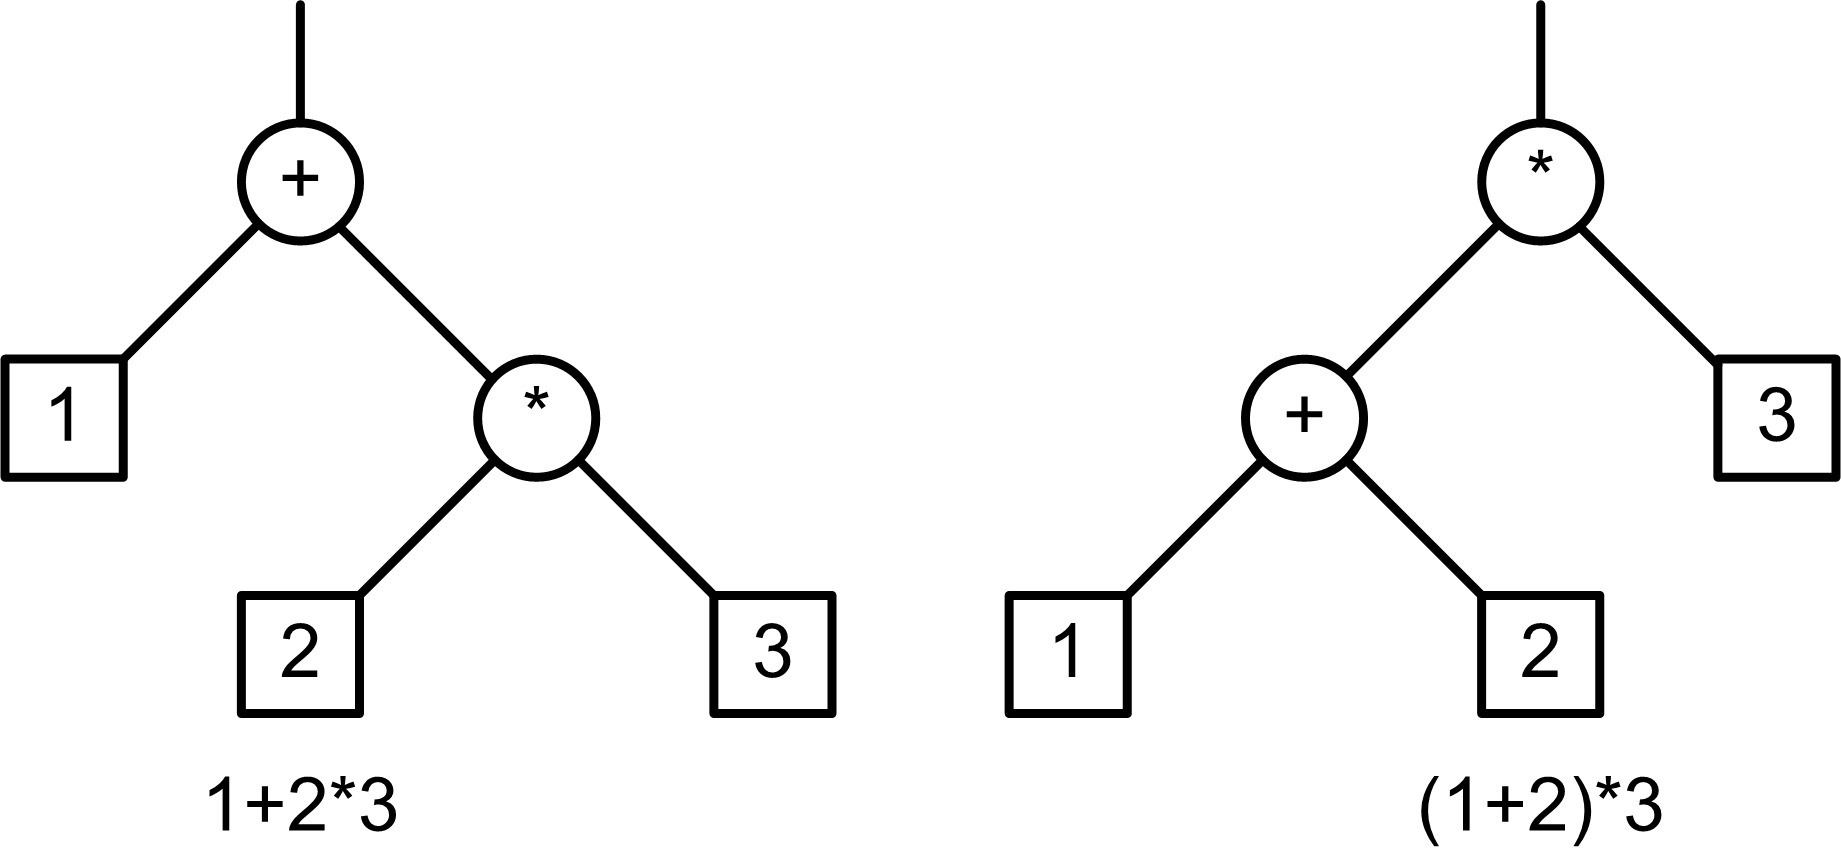
\includegraphics[width=0.67\textwidth]{fig/formulaeTree.png}
        \caption{Пример соответствия дерева формуле}\label{fig:rec:formulaeTree}
    \end{figure}
    
    Так как по принятым соглашениям умножение выполняется раньше, то формуле $1+2*3$ эквивалентна формула $(1+(2*3))$, а формуле $(1+2)*3$ --- формула $((1+2)*3)$. Соответствующие деревья приведены на рисунке \ref{fig:rec:formulaeTree}.
\end{proof}

Привычная запись формул называется \emph{инфиксной}. Проводить вычисления по инфиксной записи не удобно: на порядок действий влияют, например, приоритет, скобки и ассоциативнось операций. Более удобной для вычислений является запись \emph{постфиксная} запись\footnote{Постфиксную запись часто называют польской записью}, не содержащая ни скобок, ни других условностей. Получение постфиксной записи формулы из соответствующего дерева приведено в псевдокоде \ref{alg:rec:postfix}. Псевдокод для инфиксной и постфиксной форм будет отличаться от псевдокода \ref{alg:rec:postfix} лишь в строке \ref{alg:l:rec:sOrder}.
\begin{itemize}
    \item Для инфиксной формы: $s\gets \text{<<(>>}s_1s_3s_2\text{<<)>>}$.
    \item Для префиксной формы: $s\gets s_3s_1s_2$.
\end{itemize}

\begin{algorithm}
    \caption{Постфиксная запись формулы $postfix(t)$}\label{alg:rec:postfix}
    \begin{algorithmic}[1]
        \REQUIRE{$t$ --- дерево, соответствующее формуле. $t.text$ --- содержимое узла, $t.left$ --- левое поддерево, $t.right$ --- правое поддерево}
        \ENSURE{$s$ --- постфиксная запись формулы}

        \IF{$t$ --- отдельный узел}
            \STATE{$s\gets t.text$}
        \ELSE[$t$ содержит поддеревья]
            \STATE{$s_1\gets postfix(t.left)$} 
            \STATE{$s_2\gets postfix(t.right)$}
            \STATE{$s_3\gets t.text$}
            \STATE{$s\gets s_1s_2s_3$}\label{alg:l:rec:sOrder}
        \ENDIF
        \RETURN{$s$}
    \end{algorithmic}
\end{algorithm}

Рекурсивный обход дерева формулы $1+2*3$ и получение префиксной, инфиксной и постфиксной форм представлен на рисунке \ref{fig:rec:XfixForms}.

\begin{figure}
    \centering
    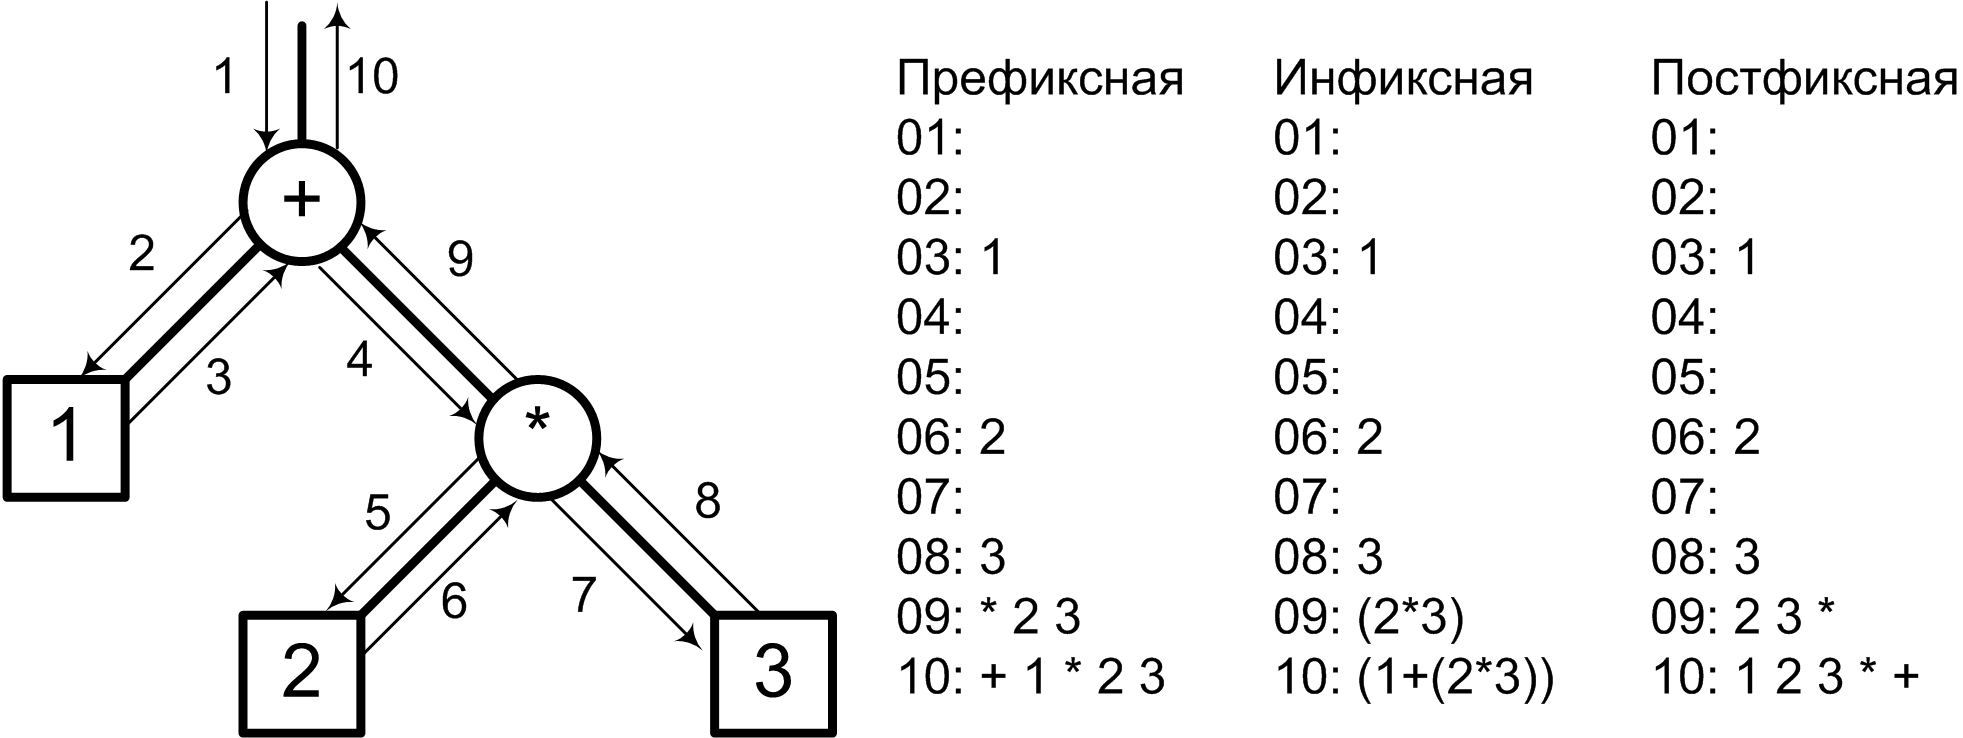
\includegraphics[width=0.87\textwidth]{fig/XfixForms.png}
    \caption{Префиксная, инфиксная и постфиксная запись $1+2*3$}
    \label{fig:rec:XfixForms}
\end{figure}

С вычислением постфиксной записи формулы спрвляется \emph{стековая машина}\footnote{Популярная виртуальная машина java является стековой}. \emph{Стек} --- это магазинная память, доступ к которой осуществляется с помощью двух команд:
\begin{enumerate}
    \item $push(X)$ --- поместить значение $X$ на вершину стека;
    \item $pop()$ --- изьять с вершины стека значение и вернуть его; $Y=pop()$ --- в $Y$ получим значение с вершины стека.
\end{enumerate}

Стек работает по принципу <<последним пришел, первым ушел>> (LIFO --- Last In First Out). То есть элементы, помещенные в стек командами $push$ будут извлечены в обратном порядке командами $pop$.

Алгоритм работы стековой машины для интерпретации постфиксной записи будет таким.
\begin{itemize}
    \item Вход: программа в виде выражения в постфиксной (обратной польской) записи.
    \item Выход: результат вычисления выражения.
    \item Шаги.
    \begin{enumerate}
        \item Программа просматривается посимвольно слева направо. Указатель текущего символа $ip$ устанавливается на начало программы.
        
        \item \label{en:rec:stackSee}Если текущий символ --- число или идентификатор переменной (обозначим и то и другое $X$), то соответствующее значение помещается в стек: $push(X)$, указатель текущего символа смещается вправо и выполняется перход на шаг \ref{en:rec:stackSee}. Иначе --- переход к следующему шагу.
        
        \item Если текущий символ выражения --- символ операции, то из стека командами $pop()$ извлекается необходимое количество аргументов, над которыми выполняется соответствующая операция, результат $R$ помещается в стек: $push(R)$, а указатель текущего символа сдвигается вправо и выполняется переход на шаг \ref{en:rec:stackSee}. Иначе --- к следующему шагу.
        
        \item Завершение работы. Достигнут конец выражения, а на вершине стека получен результат: $R=pop()$.
    \end{enumerate}
\end{itemize}

Работа стековой машины проиллюстрирована на рисунке \ref{fig:rec:stackMachine}.

\begin{figure}
    \centering
    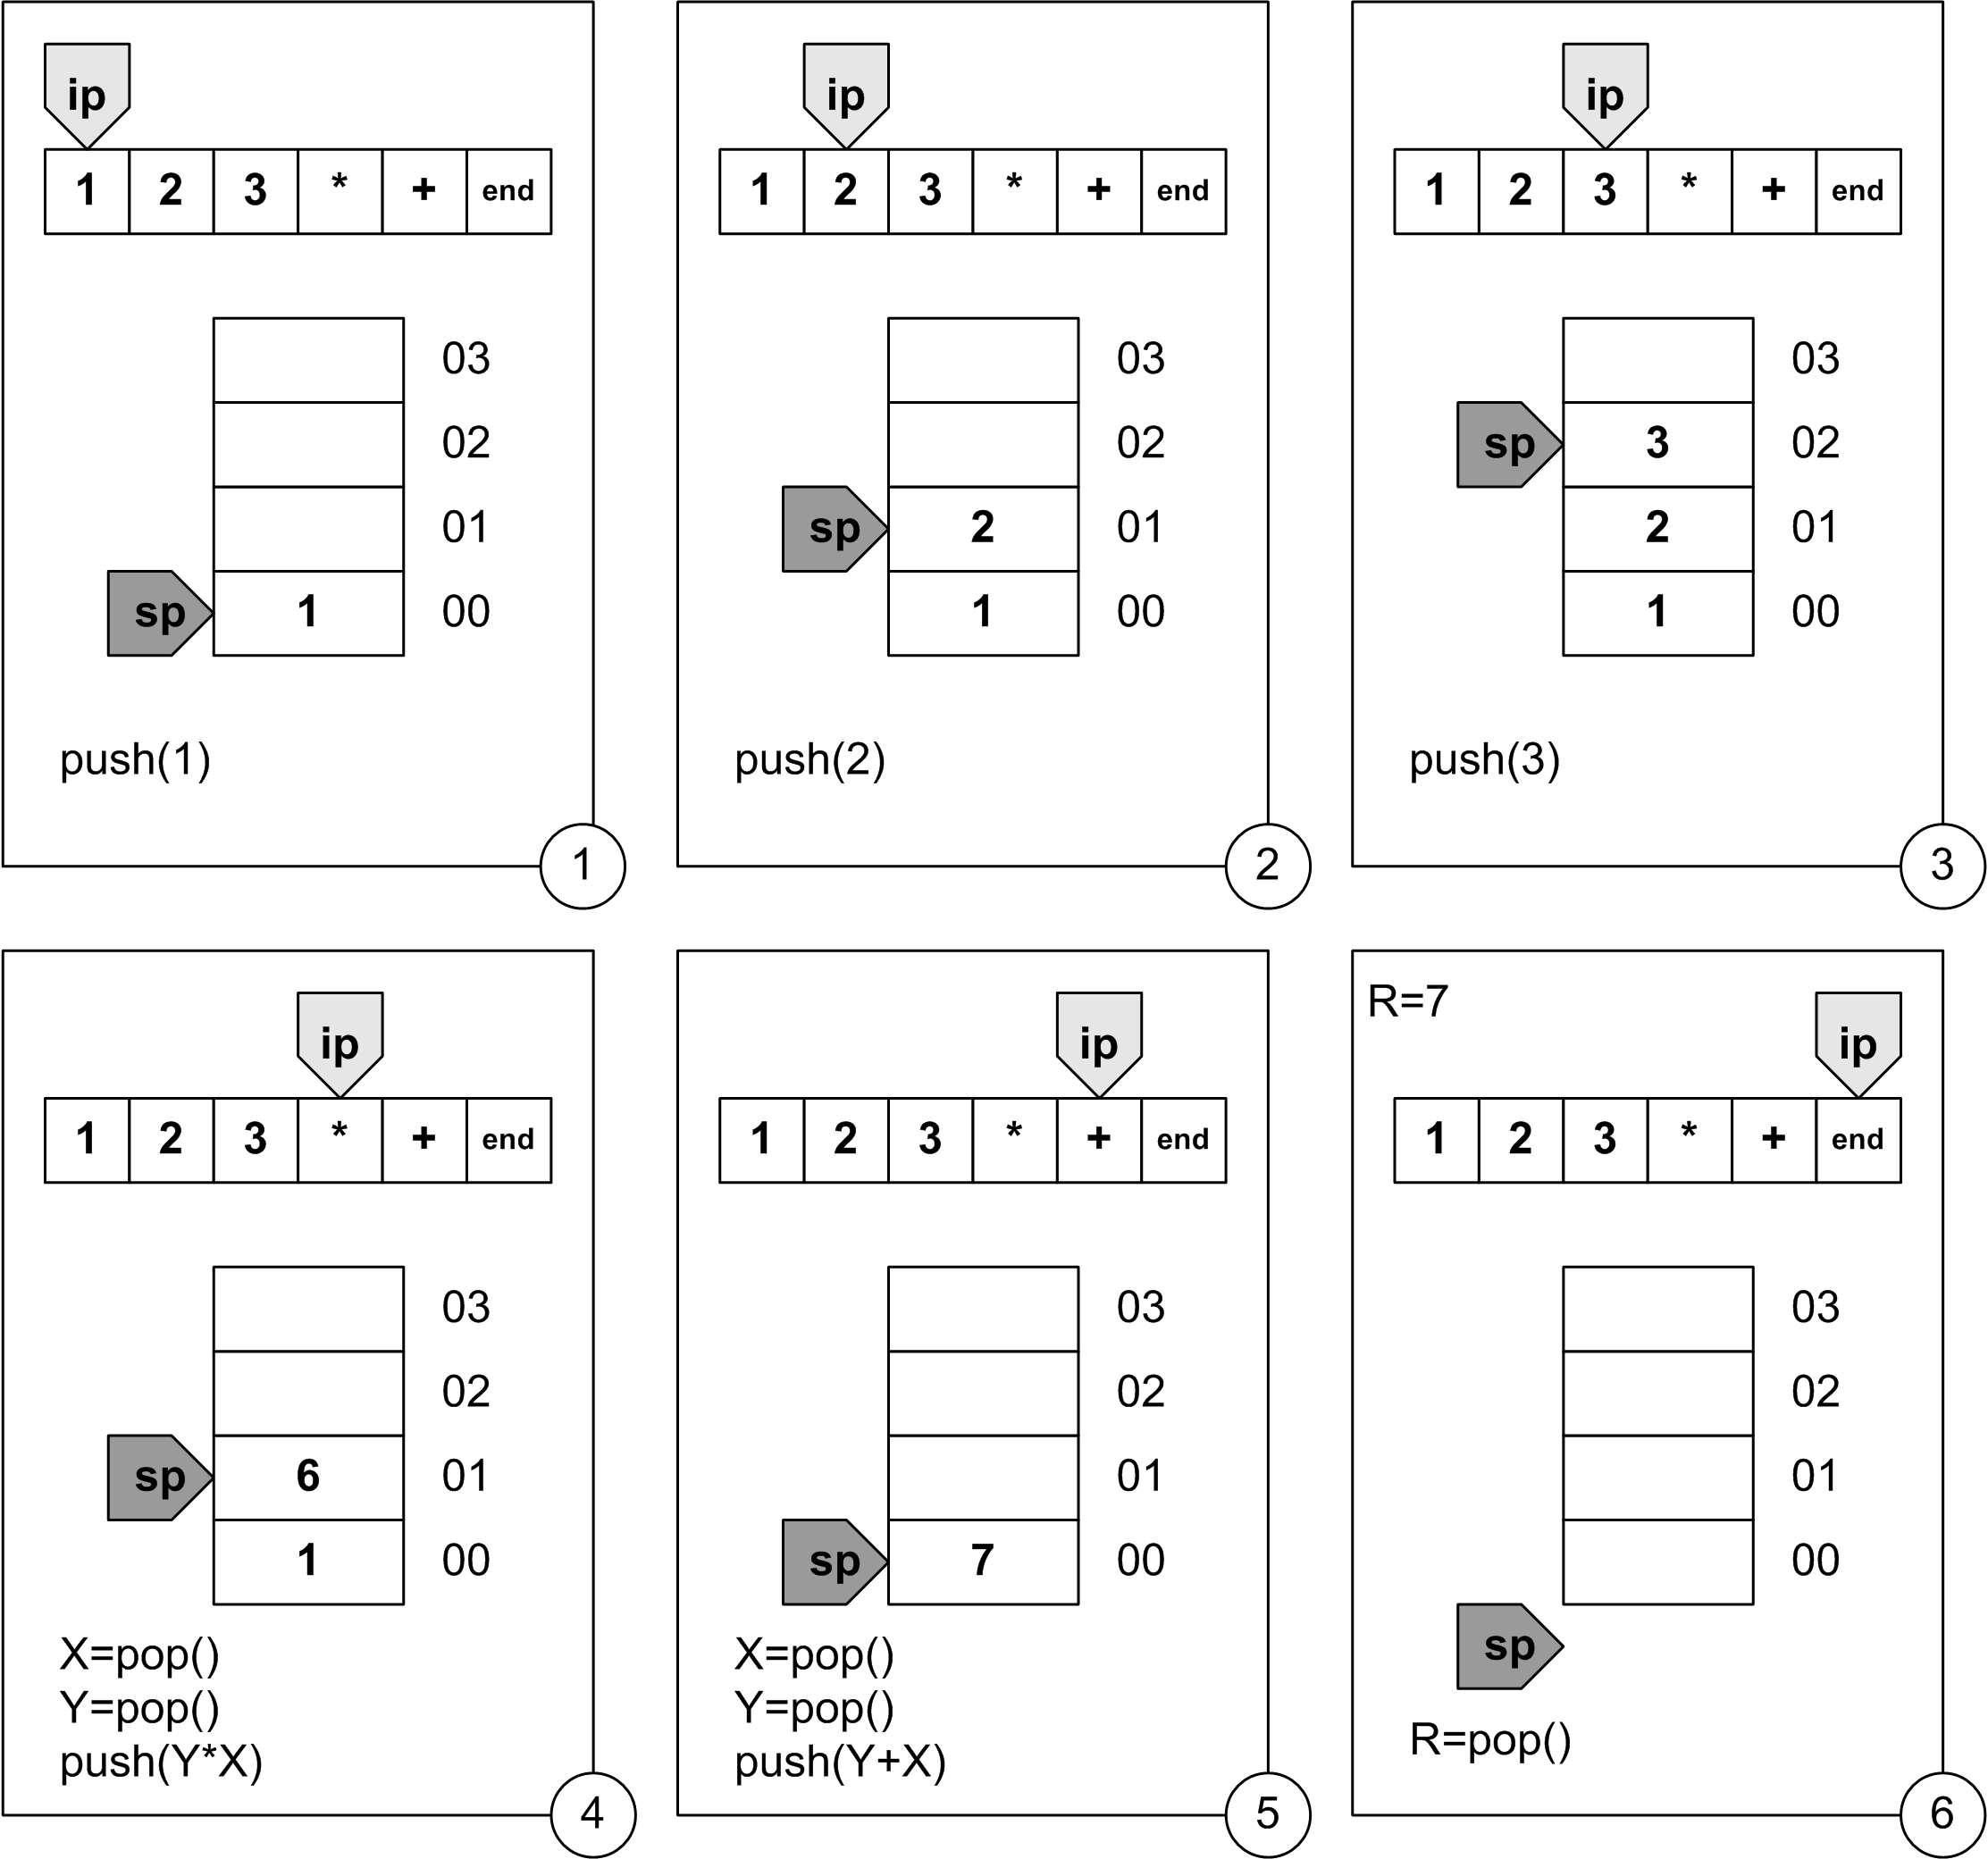
\includegraphics[width=0.87\textwidth]{fig/stackMachine.png}
    \caption{Стековая машина интерпретирует постфиксную запись}
    \label{fig:rec:stackMachine}
\end{figure}


\section{Представление деревьев в ЭВМ}

В качестве примера выбрано дерево, представленное на рисунке \ref{fig:rec:treeRepBase}. Дальнейшие примеры представления деревьев эквивалентны ему.
\begin{figure}
    \centering
    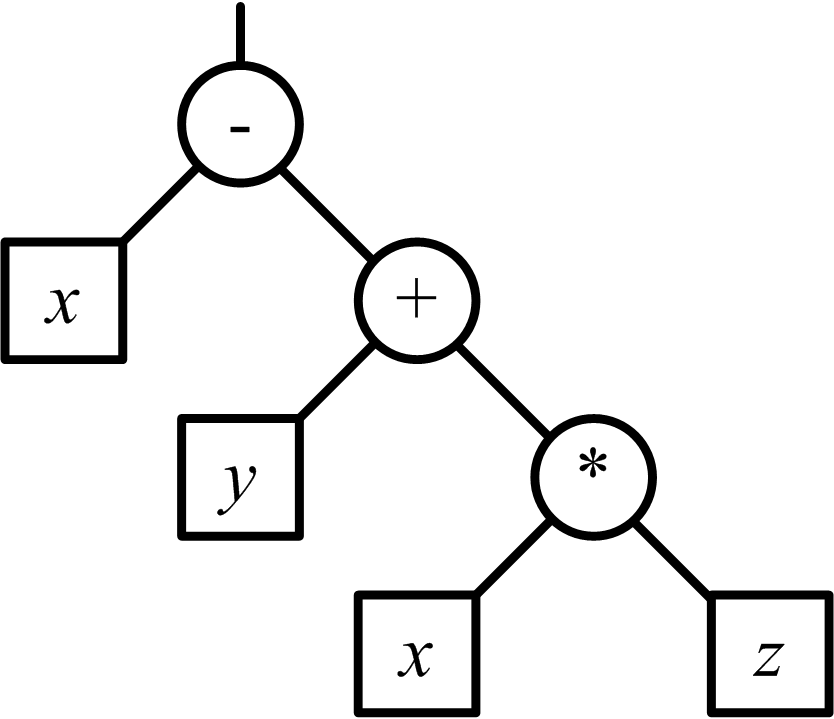
\includegraphics[width=0.3\textwidth]{fig/treeRepBase.png}
    \caption{Дерево для $x-(y+x*z)$}
    \label{fig:rec:treeRepBase}
\end{figure}


\subsection{Представление деревьев в памяти}

Дерево в памяти ЭВМ очевидным способом представляется структурой $T$, которая содержит полезные данные узла-корня и мaссив \emph{ссылок} на структуры $T$. В памяти, поддеревья, состоящие из одного узла, содержат специальное значение <<пустой>> ссылки (null) во всех элементах массива ссылок на структуры $T$. В программе дерево представлено ссылкой на корневую структуру $T$ дерева. См. рис. \ref{fig:rec:treeRepList}. 
\begin{figure}
    \centering
    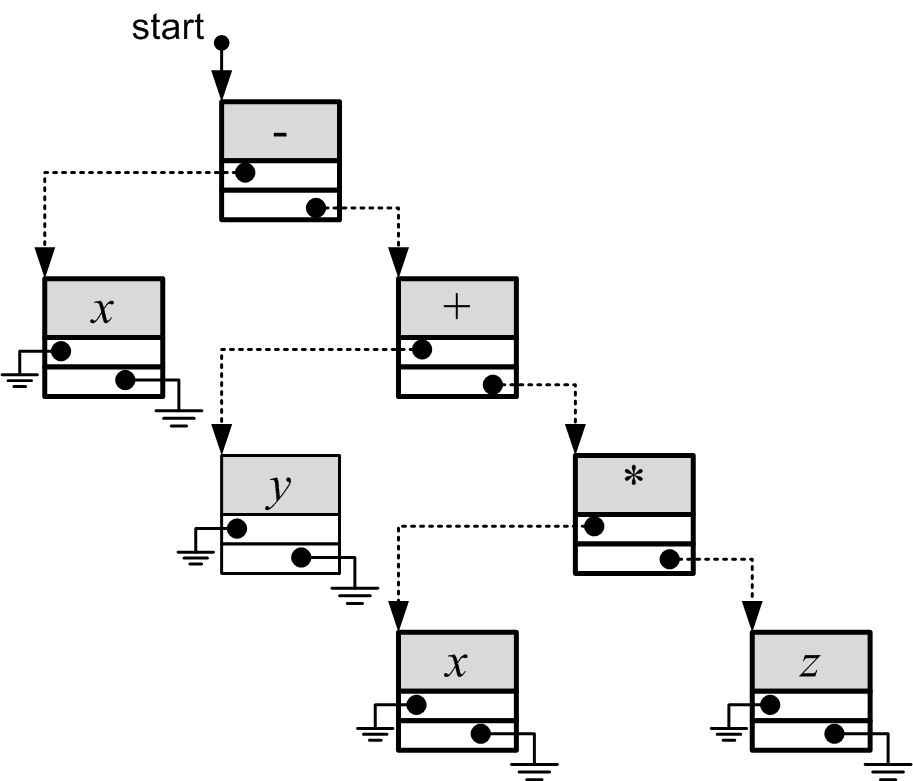
\includegraphics[width=0.57\textwidth]{fig/treeRepList.png}
    \caption{Представление дерева двусвязным списком}
    \label{fig:rec:treeRepList}
\end{figure}

В ряде задач требуется представить эквивалент дерева в виде линейного списка или массива, чтобы упростить обход. В этом случае можно предложить следующее представление. Модифицировав псевдокод \ref{alg:rec:postfix} постфиксной записи так, чтобы выражения выводились в скобках, для дерева на рис. \ref{fig:rec:treeRepBase} получим следующий список:
\[
    ((x)((y)((x)(z)*)+)-).
\]
В памяти его удобно представить массивом (списком см. рис. \ref{fig:rec:treeRepLinearList}) структур $N=\langle l,n,r\rangle$, где $n$ --- значение узла, $l$ --- количество открывающих скобок слева, $r$ --- количество закрывающих скобок справа:
\[
    \langle 2,x,1\rangle,
    \langle 2,y,1\rangle, 
    \langle 2,x,1\rangle,
    \langle 1,z,1\rangle,
    \langle 0,*,1\rangle,
    \langle 0,+,1\rangle,
    \langle 0,-,1\rangle.
\]

\begin{figure}
    \centering
    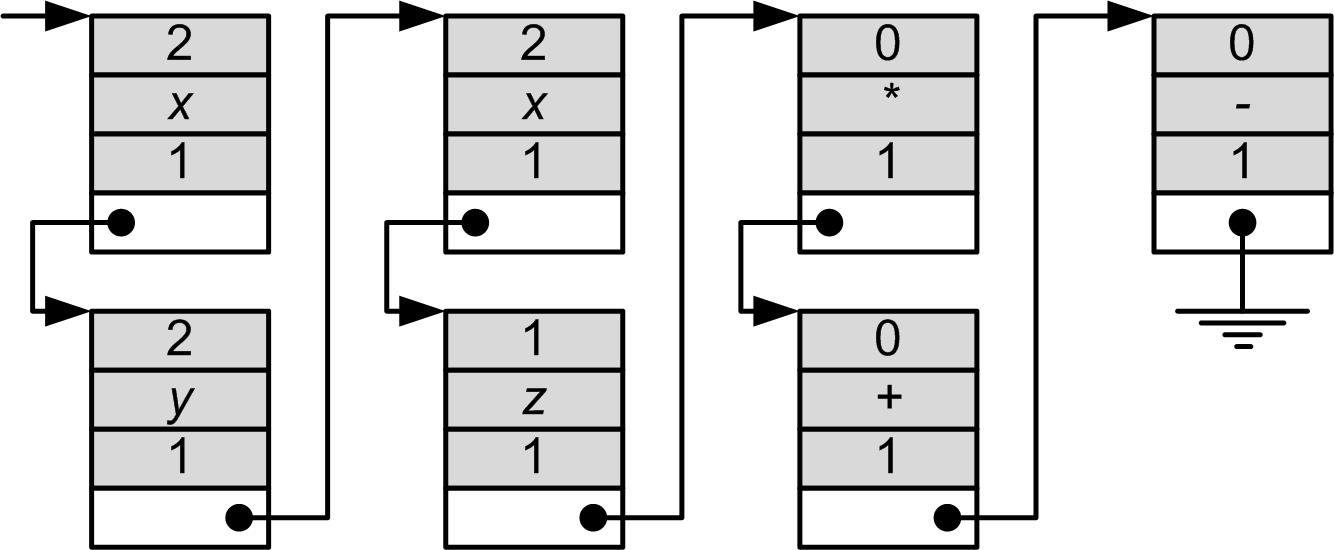
\includegraphics[width=0.57\textwidth]{fig/treeRepLinearList}
    \caption{Представление дерева линейным списком}
    \label{fig:rec:treeRepLinearList}
\end{figure}

Конечно, возможны и другие представления деревьев в памяти.


\subsection{Представление деревьев в реляционных таблицах}

Таблицы реляционных баз данных предназначены для хранения отношений, но иногда требуется представить в табличном виде дерево. Наиболее простой способ это сделать (см. рис. \ref{fig:rec:treeRepParent}) --- проиндексировать узлы дерева и в соответствующей таблице определить поля:
\begin{itemize}
    \item идентификатор узла (id);
    \item значение узла (text);
    \item идентификатор родительского узла (pid).
\end{itemize}

При этом идентификатор родительского узла корня совпадает с его собственным идентификатором.
\begin{figure}
    \centering
    \begin{tabular}{cc}
        \begin{tabular}{|c|c|c|}
            \hline\hline
            id  &text   &pid \\
            \hline\hline
            1   &-      &1 \\ \hline
            2   &x      &1 \\ \hline
            3   &+      &1 \\ \hline
            4   &y      &3 \\ \hline
            5   &*      &3 \\ \hline
            6   &x      &5 \\ \hline
            7   &z      &5 \\ \hline
        \end{tabular}
        &\raisebox{-.5\height}{
            \fbox{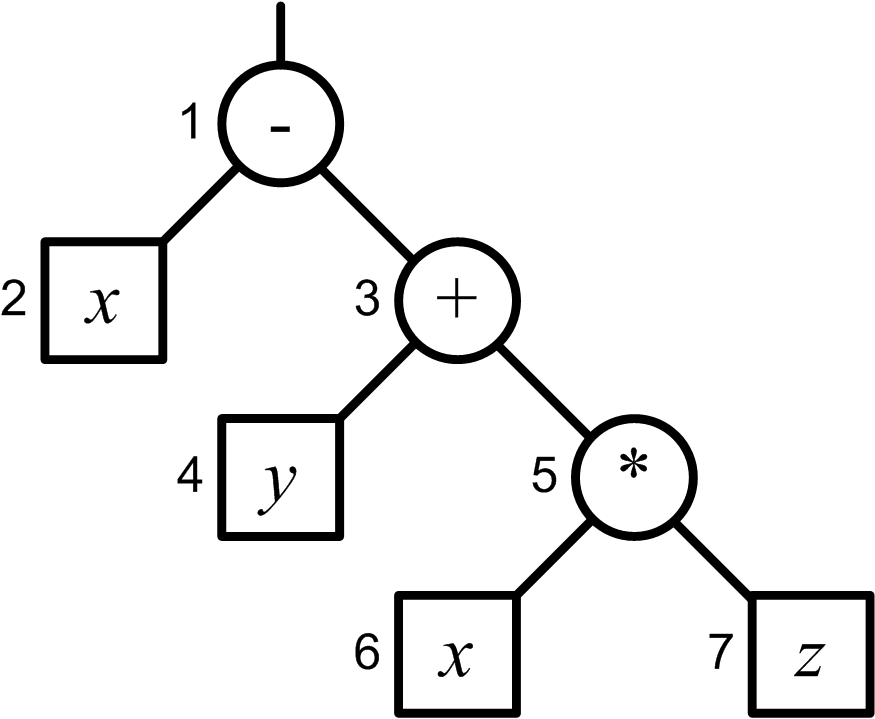
\includegraphics[width=0.3\textwidth]{fig/treeRepParent.png}}
        }
    \end{tabular}
    \caption{Табличное преставление с помощью ссылок на родительский узел}
    \label{fig:rec:treeRepParent}
\end{figure}

При этом для поиска корня дерева можно использовать запрос
\begin{verbatim}
select * from tree where id=pid;
\end{verbatim}

Поиск всех дочерних узлов для узла с известным идентификатором \verb"ID" организуется также весьма просто:
\begin{verbatim}
select * from tree where pid=:ID;
\end{verbatim}

Найти предка, если известен параметр \verb"PID" потомка также весьма просто:
\begin{verbatim}
select * from tree where pid=:PID;
\end{verbatim}

Но вот определить все узлы поддеревьев некоторого узла можно только рекурсивно. Эту проблему решает представление с помощью \emph{вложенных множеств}. Проведя уже знакомую модификацию псевдокода \ref{alg:rec:postfix} легко получим для дерева списочное представление в постфиксной записи. При этом для каждой скобки верхним индексом поставим её вложенность, а нижним --- её номер по порядку:
\[
    \Big(_0^1
        \Big(_1^2 x\Big)_2^2\ 
        \Big(_3^2
            \Big(_4^3 y\Big)_5^3\ 
            \Big(_6^3
                \Big(_7^4 x\Big)_8^4\ 
                \Big(_9^4 z\Big)_{10}^4 *
            \Big)_{11}^3 +
        \Big)_{12}^2 -
    \Big)_{13}^1.
\]

В соответствующей таблице (см. рис. \ref{fig:rec:treeRepNested}) следует определить поля:
\begin{itemize}
    \item значение узла (text);
    \item уровень вложенности (верхний индекс скобок) узла (lvl);
    \item номер (нижний индекс) открывающей скобки узла (l);
    \item номер (верхний индекс) закрывающей скобки узла (r).
\end{itemize}

\begin{figure}
    \centering
    \begin{tabular}{cc}
        \begin{tabular}{|c|c|c|c|}
            \hline\hline
            text&lvl    &l      &r \\
            \hline\hline
            +   &2      &3      &12 \\ \hline
            -   &1      &0      &13 \\ \hline
            *   &3      &6      &11 \\ \hline
            x   &2      &1      &2  \\ \hline
            x   &4      &7      &8  \\ \hline
            y   &3      &4      &5  \\ \hline
            z   &4      &9      &10 \\ \hline
        \end{tabular}
        &\raisebox{-.5\height}{\fbox{
            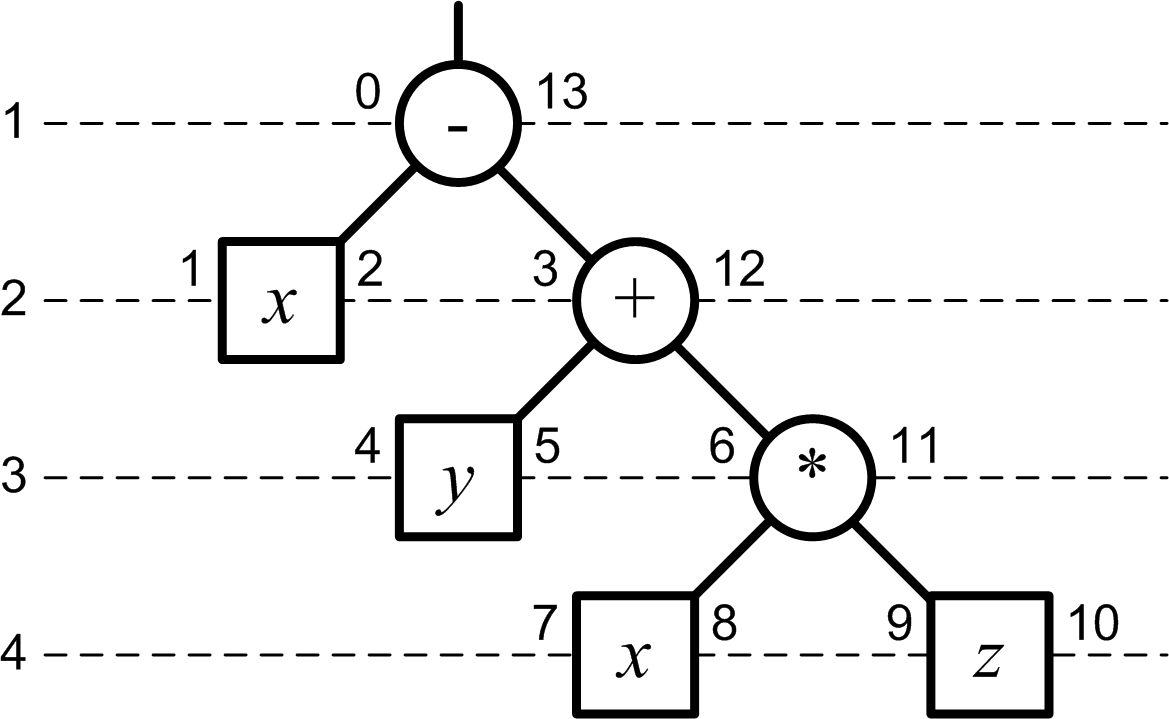
\includegraphics[width=0.4\textwidth]{fig/treeRepNested.png}
        }}
    \end{tabular}
    \caption{Табличное преставление с помощью вложенных множеств}
    \label{fig:rec:treeRepNested}
\end{figure}

Теперь, если известны параметры \verb"LVL", \verb"L", \verb"R" узла то запрос на получение непосредственных потомков будет выглядеть так:
\begin{verbatim}
select * from tree where lvl=:LVL+1 and l>:L and r<:R;
\end{verbatim}

Найти предка можно запросом
\begin{verbatim}
select * from tree where lvl=:LVL-1 and l<:L and r>:R;
\end{verbatim}

Для того, чтобы выбрать все узлы поддеревьев узла достаточно снять ограничение на уровень вложенности:
\begin{verbatim}
select * from tree where l>:L and r<:R;
\end{verbatim}

Приведенные выше способы не накладывают ограничений на глубину дерева. В ряде случаев максимальная глубина дерева известна. Тогда можно воспользоваться следующим рекурсивным способом индексирования вершин дерева.
\begin{enumerate}
    \item База. Корень дерева получает индекс $1$.
    \item Рекурсивный переход. Для всех узлов-потомков $a_1,\ldots,a_n$ некоторого узла с индексом $i$ соответствующие индексы будут $i.1,\ldots,i.n$.
\end{enumerate}

В таблице, кроме поля значения узла (text), отводится соответствующее количество полей (i1,i2,\ldots) для индексов каждого уровня (см. рис. \ref{fig:rec:treeRepConstLevel}).

\begin{figure}
    \centering
    \begin{tabular}{cc}
        \begin{tabular}{|c|c|c|c|c|c|}
            \hline\hline
            text    &i1     &i2     &i3     &i4     &i5 \\
            \hline\hline
            -       &1      &0      &0      &0      &0 \\ \hline
            *       &1      &2      &2      &0      &0 \\ \hline
            +       &1      &2      &0      &0      &0 \\ \hline
            x       &1      &1      &0      &0      &0 \\ \hline
            x       &1      &2      &2      &1      &0 \\ \hline
            y       &1      &2      &1      &0      &0 \\ \hline
            z       &1      &2      &2      &2      &0 \\ \hline
        \end{tabular}
        &\raisebox{-.5\height}{\fbox{
            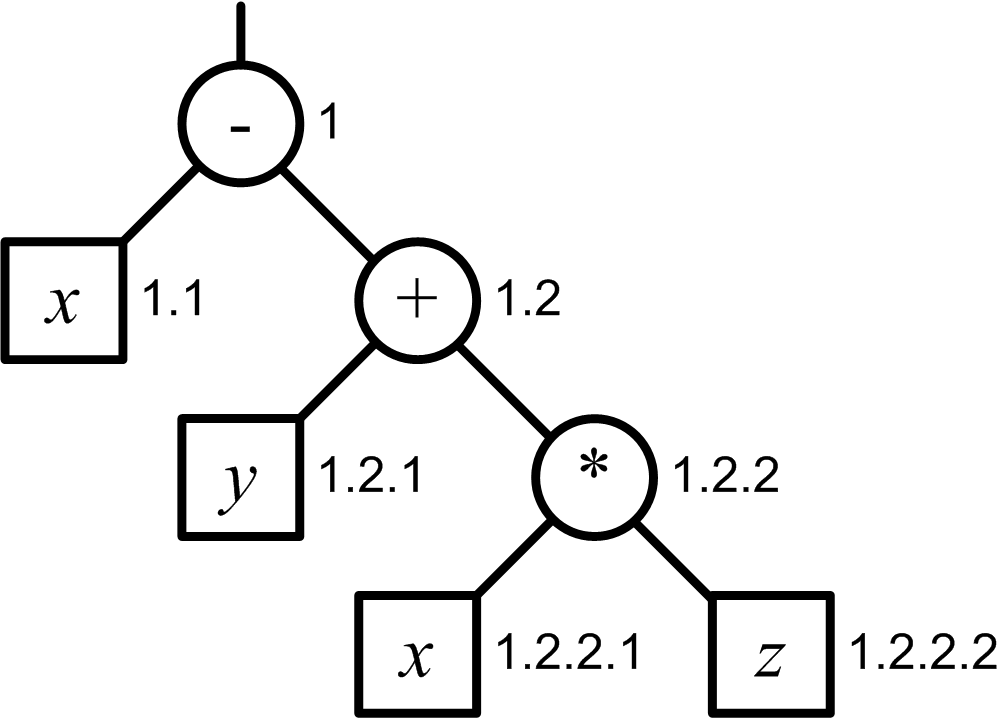
\includegraphics[width=0.35\textwidth]{fig/treeRepConstLevel.png}
        }}
    \end{tabular}
    \caption{Табличное преставление индексов узлов}
    \label{fig:rec:treeRepConstLevel}
\end{figure}

Запрос всех непосредственных потомков узла с индексом, например, <<1.2>> будет таким
\begin{verbatim}
select * from tree where i1=1 and i2=2 and i3<>0 and i4=0;
\end{verbatim}

Все узлы поддеревьев можно найти запросом
\begin{verbatim}
select * from tree where i1=1 and i2=2 and i3<>0;
\end{verbatim}

Запрос предка узла с индексом, например, <<1.2.2>> будет таким
\begin{verbatim}
select * from tree where i1=1 and i2=2 and i3=0;
\end{verbatim}

Каждый способ табличного представления деревьев имеет свои достоинства и недостатки, которые особенно остро проявляются в случае, если требуется модифицировать дерево.


\section{Рекурсивные алгоритмы}

Рекурсивный алгоритм бинарного поиска приведен в псевдокоде \ref{alg:rec:binSearchRec}. Суть алгоритма в том, что текущий диапазон массива $a[l:r]$ делится пополам. Если элемент в середине этого диапазона $a[m]$ не является искомым, то поиск продолжается либо в левой половине диапазона $a[l:m-1]$, либо в правой $a[m+1:r]$, в зависимости от результата сравнения $a[m]$ с искомым $x$.

Бинарный поиск можно выполнить итеративно (см. псевдокод \ref{alg:rec:binSearchIter}).

\begin{algorithm}
    \caption{binarySearch($a$, $x$, $l$, $r$) --- рекурсивный алгоритм бинарного поиска}
    \label{alg:rec:binSearchRec}
    \begin{algorithmic}[1]
        \REQUIRE{$a$ --- отсортированный по возрастанию массив элементов линейно упорядоченного множества. Длина массива $n$, обращение к элементу по $i$-му индексу: $a[i]$. Первый элемент массива $a[0]$, последний $a[n-1]$. Если $i\geq j$, то $a[i]\geq a[j]$. $l$ --- индекс левой границы, $r$ --- индекс правой границы. $x$ --- искомый элемент. Первый вызов: binarySearch($a$, $x$, $0$, $n-1$)}
        \ENSURE{Индекс найденного элемента. Если элемент не найден, возвращается индекс, равный $-1$.}

        \IF{$l>r$}
            \RETURN{$-1$}
        \ELSE
            \STATE{$m\gets \lfloor\frac{l+r}{2}\rfloor$} 
            \COMMENT{индекс середины диапазона $a[l:r]$}
            \IF{$x=a[m]$}
                \RETURN{$m$}
            \ELSE
                \IF{$x<a[m]$}
                    \RETURN{binarySearch($a$, $x$, $l$, $m-1$)}
                    \COMMENT{поиск в левой половине}
                \ELSE
                    \RETURN{binarySearch($a$, $x$, $m+1$, $r$)}
                    \COMMENT{поиск в правой половине}
                \ENDIF
            \ENDIF
        \ENDIF

    \end{algorithmic}
\end{algorithm}

\begin{algorithm}
    \caption{binarySearch($a$, $x$, $l$, $r$) --- итеративный алгоритм бинарного поиска}
    \label{alg:rec:binSearchIter}
    \begin{algorithmic}[1]
        \WHILE{$l\leq r$}
            \STATE{$m\gets \lfloor\frac{l+r}{2}\rfloor$} 
            \IF{$x=a[m]$}
                \RETURN{$m$}
            \ELSE
                \IF{$x<a[m]$}
                    \STATE{$r\gets m-1$} 
                \ELSE
                    \STATE{$l\gets m+1$} 
                \ENDIF
            \ENDIF
        \ENDWHILE
        \RETURN{$-1$}
    \end{algorithmic}
\end{algorithm}

На практике всегда, когда есть выбор между эквивалентными рекурсивной и итеративной версиями, выбирают версию итеративную. Рекурсивный алгоритм всегда можно свести к итеративному. В худшем случае этот итеративный алгоритм будет использовать стек, и тогда от красоты и наглядности рекурсивного решения не останется ничего. В этом случае, пожалуй стоит подумать над тем, чтобы использовать именно рекурсивное решение.

Пример с бинарным поиском весьма неудачен, потому что он не иллюстрирует основную стратегию рекурсии: \emph{разделяй и властвуй}! Да, пространство поиска разделялось на две части, но властвовали мы только над одной из них. Более удачный пример --- \emph{сортировка слиянием}. Если два массива упорядочены, то объединить их в один массив достаточно просто (см. псевдокод \ref{alg:rec:split}). Суть сортировки слиянием в том, что исходный неотсортированный массив разбивается на две части, которые рекурсивно сортируются по отдельности и затем эти части сливаются в один отсортированный массив (см. псевдокод \ref{alg:rec:splitSort}).

\begin{algorithm}
    \caption{split($a$, $l$, $m$, $r$) --- алгоритм слияния двух упорядоченных по возрастанию массивов}
    \label{alg:rec:split}
    \begin{algorithmic}[1]
    
        \REQUIRE{$a$ --- массив, содержащий две упорядоченные по возрастанию части $a[l:m-1]$ и $a[m:r]$}
        \ENSURE{Часть массива $a[l:r]$, элементы которой упорядочены по возрастанию}
    
        \WHILE{$l<m$ \AND $m\leq r$}
            \IF{$a[l]\leq a[m]$}
                \STATE{$l\gets l+1$} 
            \ELSE
                \STATE{$t\gets a[m]$} 
                \FOR{$i=m-1$ to $l$}
                    \STATE{$a[i+1]\gets a[i]$} 
                \ENDFOR
                \STATE{$a[l]\gets t$} 
                \STATE{$l\gets l+1$} 
                \STATE{$m\gets m+1$} 
            \ENDIF
        \ENDWHILE
    \end{algorithmic}
\end{algorithm}

\begin{algorithm}
    \caption{splitSort($a$, $l$, $r$) --- сортировка слиянием}
    \label{alg:rec:splitSort}
    \begin{algorithmic}[1]
    
        \REQUIRE{$a$ --- массив, элементы $a[l:r]$ которого нужно упорядочить по возрастанию. Первый элемент массива $a[0]$, последний $a[n-1]$. Первый вызов: splitSort($a$, $0$, $n-1$)}
        \ENSURE{Массив $a$, элементы которого упорядочены по возрастанию}
    
        \IF{$l<r$}
            \STATE{$m\gets \lfloor\frac{l+r}{2}\rfloor$} \COMMENT{разделяем}
            \STATE{splitSort($a$, $l$, $m$)} \COMMENT{властвуем}
            \STATE{splitSort($a$, $m+1$, $r$)} \COMMENT{властвуем}
            \STATE{split($a$, $l$, $m+1$, $r$)} \COMMENT{объединяем решения}
        \ENDIF
    \end{algorithmic}
\end{algorithm}

Ход сортировки массива процедурой splitSorn представлен на рисунке \ref{fig:rec:splitSortEx}.
\begin{figure}
\[
\resizebox{\textwidth}{!}
{
    {\xymatrix{
        *{}
            &*{}
                &*{}
                    &*{}
                        &*{}
                            &*{}
                                &*{}
                                    &*{\fbox{4\,1\,9\,5\,2\,6\,8\,3}}\ar@{-}[dllll]\ar@{-}[drrrr]
                                        &*{}
                                            &*{}
                                                &*{}
                                                    &*{}
                                                        &*{}
                                                            &*{}
                                                                &*{}
                                                                    \\
        *{}
            &*{}
                &*{}
                    &*{\fbox{4\,1\,9\,5}}\ar@{-}[dll]\ar@{-}[drr]
                        &*{}
                            &*{}
                                &*{}
                                    &*{}
                                        &*{}
                                            &*{}
                                                &*{}
                                                    &*{\fbox{2\,6\,8\,3}}\ar@{-}[dll]\ar@{-}[drr]
                                                        &*{}
                                                            &*{}
                                                                &*{}
                                                                    \\
        *{}
            &*{\fbox{4\,1}}\ar@{-}[dl]\ar@{-}[dr]
                &*{}
                    &*{}
                        &*{}
                            &*{\fbox{9\,5}}\ar@{-}[dl]\ar@{-}[dr]
                                &*{}
                                    &*{}
                                        &*{}
                                            &*{\fbox{2\,6}}\ar@{-}[dl]\ar@{-}[dr]
                                                &*{}
                                                    &*{}
                                                        &*{}
                                                            &*{\fbox{8\,3}}\ar@{-}[dl]\ar@{-}[dr]
                                                                &*{}
                                                                    \\
        *{\fbox{4}}\ar@{-}[dr]
            &*{}
                &*{\fbox{1}}\ar@{-}[dl]
                    &*{}
                        &*{\fbox{9}}\ar@{-}[dr]
                            &*{}
                                &*{\fbox{5}}\ar@{-}[dl]
                                    &*{}
                                        &*{\fbox{2}}\ar@{-}[dr]
                                            &*{}
                                                &*{\fbox{6}}\ar@{-}[dl]
                                                    &*{}
                                                        &*{\fbox{8}}\ar@{-}[dr]
                                                            &*{}
                                                                &*{\fbox{3}}\ar@{-}[dl]
                                                                    \\
        *{}
            &*{\fbox{1\,4}}\ar@{-}[drr]
                &*{}
                    &*{}
                        &*{}
                            &*{\fbox{5\,9}}\ar@{-}[dll]
                                &*{}
                                    &*{}
                                        &*{}
                                            &*{\fbox{2\,6}}\ar@{-}[drr]
                                                &*{}
                                                    &*{}
                                                        &*{}
                                                            &*{\fbox{3\,8}}\ar@{-}[dll]
                                                                &*{}
                                                                    \\
        *{}
            &*{}
                &*{}
                    &*{\fbox{1\,4\,5\,9}}\ar@{-}[drrrr]
                        &*{}
                            &*{}
                                &*{}
                                    &*{}
                                        &*{}
                                            &*{}
                                                &*{}
                                                    &*{\fbox{2\,3\,6\,8}}\ar@{-}[dllll]
                                                        &*{}
                                                            &*{}
                                                                &*{}
                                                                    \\
        *{}
            &*{}
                &*{}
                    &*{}
                        &*{}
                            &*{}
                                &*{}
                                    &*{\fbox{1\,2\,3\,4\,5\,6\,8\,9}}
                                        &*{}
                                            &*{}
                                                &*{}
                                                    &*{}
                                                        &*{}
                                                            &*{}
                                                                &*{}
    }}
}
\]
    \caption{Пример выполнения splitSort([4,1,9,5,2,6,8,3],0,7)}
    \label{fig:rec:splitSortEx}
\end{figure}

За знаниями по основным алгоритмам можно обратится к книгам \cite{bib:wirth:alghorithms,bib:kernigan:practice}. Нельзя не сказать о фундаментальном труде Дональда Кнута \cite{bib:knuth:artOfProgramming1, bib:knuth:artOfProgramming2, bib:knuth:artOfProgramming3}. Алгоритмы с точки зрения их анализа рассматриваются в книгах \cite{bib:mcconnel:alghorithmAnalysis, bib:miller:secParAlghorithm}.


\section*{Задания}
\addcontentsline{toc}{section}{Задания}

\begin{enumerate}
    \item Доказать по индукции, что  
    \begin{enumerate}
        \item $n!>n^2$ при $n\geq 4$.
        \item $2^n>n^3$ при $n\geq 10$.
        \item $3$ делит $n^3+2n$ при $n>0$.
        \item $6$ делит $n^3-n$ при $n>0$.
        \item $\frac{1}{1\cdot 2}+\frac{1}{2\cdot 3}+\cdots+\frac{1}{n(n+1)}=\frac{n}{n+1}$ при $n\geq 1$.
        \item Формулы \eqref{eq:rec:rec1type} и \eqref{eq:rec:rec1typeSum} эквивалентны.
    \end{enumerate}

    \item Найти решение реккурентности 
    \[
        f(n)=
        \begin{cases}
            c,                  &n=0,\\
            a\cdot f(n-1) + b,  &n\geq 1
        \end{cases}
    \]
    в аналитическом виде.
    
    \item Алгоритм поиска $\text{НОД}$ --- наибольшего общего делителя (gcd\footnote{gcd --- greatest common divisor}) рекурсивно задается так:
    \[
        \text{НОД}(a,b)=
        \begin{cases}
            b,                      &a=0\\
            \text{НОД}(b \bmod a,a),&a>0
        \end{cases}
    \]
    Найдите $\text{НОД}(210,119)$
    
    \item Понятие упорядоченного набора элементов, т.е. кортежа $(a_1,a_2,\ldots,a_n)$ длины $n$ можно свести рекурсивно к понятию \emph{упорядоченной пары} (tuple):
    \[
        (a_1,\ldots,a_n)=
        \begin{cases}
            ()=\emptyset, &n=0,\\
            (a_1,a_2,\ldots,a_n)=(a_1,(a_2,\ldots,a_n)), &n>0.
        \end{cases}
    \]
    Так, например 
    \begin{itemize}
        \item $()=\emptyset$; 
        \item $(a_1)=(a_1,())=(a_1,\emptyset)$;
        \item $(a_1,a_2)=(a_1,(a_2,\emptyset))$;
        \item $(a_1,a_2,a_3)=(a_1,(a_2,(a_3,\emptyset)))$.
    \end{itemize}
    
    То есть, определяя кортеж длины $n$ можно обойтись лишь понятием упорядоченной пары. Для упорядоченной пары $(a,b)$, в отличие от множества $\{a,b\}$, характерно $(a,b)\neq(b,a)$, если $a\neq b$. Упорядоченную пару можно определить через множества\footnote{Казимир Куратовский, 1921}: $(a,b)=\{\{a\},\{a,b\}\}$. Это, в частности, означает что понятие кортежа лишь искусственный конструкт, созданный на основе множеств исключительно для удобства. Тогда, объединяя вышеизложенное, можно определить кортеж длины $n$ так:
    \[
        (a_1,\ldots,a_n)=
        \begin{cases}
            ()=\emptyset, &n=0,\\
            (a_1,a_2,\ldots,a_n)=\{\{a_1\},\{a_1, (a_2,\ldots,a_n)\}\}, &n>0.
        \end{cases}
    \]
    
    Тогда:
    \begin{itemize}
        \item $()=\emptyset$; 
        \item $(a_1)=\{\{a_1\},\{a_1,()\}\}=\{\{a_1\},\{a_1,\emptyset\}\}$;
        \item $(a_1,a_2)=\{\{a_1\},\{a_1,(a_2)\}\}=\{\{a_1\},\{a_1,\{\{a_2\},\{a_2,\emptyset\}\}\}\}$.        
    \end{itemize}

    Задание
    \begin{enumerate}
        \item Найти представление множеством кортежа $(a_1,a_2,a_3)$;
        \item Написать программу для нахождения представления произвольного кортежа множеством;
        \item Определить, какому кортежу соответствует $\{\{\emptyset\}\}$;
        \item Определить, какому кортежу соответствует 
        \begin{enumerate}
            \item $\{\{b,\{\{a,\emptyset\},\{a\}\}\},\{b\}\}$;
            \item $\{\{a,\{\{c,\{\{b,\emptyset\},\{b\}\}\},\{c\}\}\},\{a\}\}$;
            \item $\{\{d,\{\{a,\{\{c,\{\{b,\emptyset\},\{b\}\}\},\{c\}\}\},\{a\}\}\},\{d\}\}$.
        \end{enumerate} 
        \item Написать программу для нахождения кортежа по представлению множеством, с учетом того, что $\{a,b\}=\{b,a\}$. Значениями координат кортежа могут быть лишь одиночные символы. Пустое множество значением координаты быть не может.
    \end{enumerate}
    
    \item Решить задачу разрезания торта: сколько кусков торта можно получить, делая $n$ прямолинейных разрезов ножом. Усложните задачу, предполагая, что торт разрезается двумя прямолинейными резами, исходящими из одной точки.
    
    \item Построить дерево, постфиксную и префиксную запись выражения в инфиксной форме:
    \begin{enumerate}
        \item $(a+b/c)*(d-e*f)$;
        \item $(a+b-c)*(d+e)*f$;
        \item $(a+b-c)*(d+e)-f$;
        \item $(a+b/c)-(d-e)*f$;
        \item $(a+b)/c-d/e*f$;
        \item $(a+b)/(c-(d-e)*f)$.
    \end{enumerate}
    
    \item Преобразовать в инфиксную форму выражения в постфиксной форме:
    \begin{enumerate}
        \item $abc+d*-$;
        \item $ab+c-d*$;
        \item $ab*cd+e-+$;
        \item $ab+cde-+*$;
        \item $abc-*de+-$;
        \item $abc/*de+-$.
    \end{enumerate}

    \item Представить дерево в табличном виде с помощью вложенных множеств, соответствующее формуле:
    \begin{enumerate}
        \item $(a+b/c)*(d-e*f)$;
        \item $(a+b-c)*(d+e)*f$;
        \item $(a+b-c)*(d+e)-f$;
        \item $(a+b/c)-(d-e)*f$;
        \item $(a+b)/c-d/e*f$;
        \item $(a+b)/(c-(d-e)*f)$.
    \end{enumerate}

    \item Напишите псевдокод для вычисления $n$-го числа Фибоначчи рекурсивно и итеративно. Оцените какой алгоритм будет работать быстрее.
\end{enumerate}
